
\section{$\psi_{\rho}$ 的构造}
\label{sec:construction-psi-rho}

对每个 $\rho\ge\rho_{0}$，我们已经构造了一个属于 $\cC^{\infty}(x,z)$ 的 $w_{\rho}$，并且由于\trExponentialDecay{}（\cref{sec:exponential-decay}），它甚至是 $\cC^{\infty}_{\searrow}(x,z)$ 中的一个元素。现在我们要对每个 $\rho\ge\rho_{0}$ 定义一个 $\psi_{\rho}\in\scr{M}(x,z)$（这一次是一个真正的解），它将具有形式
\[
\psi_{\rho}=\exp_{w_{\rho}}\gamma(\rho)\qquad\text{其中 }\gamma(\rho)\in T_{w_{\rho}}\scr{P}(x,z)=W^{1,p}(w_{\rho}^{\star}TW)\text{，}
\]

\begin{remark}\label{thm:floer-operator-weak-sense}
一如既往，我们让 $\scr{F}$ 表示“\trFloer”算子
\[
\scr{F}=\frac{\partial}{\partial s}+J\frac{\partial}{\partial t}+\operatorname{grad}H\text{。}
\]
要验证 $\psi_{\rho}$ 是一个解，只需验证 $\scr{F}(\psi_{\rho})=0$ 在弱的意义下成立就够了。的确，$\psi_{\rho}$ 将自动是连续的（由于 $\gamma(\rho)\in W^{1,p}(w_{\rho}^{\star}TW)$ 且 $p>2$，故 $\gamma(\rho)$ 连续），从而是一个强解，并且再一次应用\trEllipticRegularity{}（\cref{thm:loc-topologies-coincide}）便知它属于 $\cC^{\infty}$ 类。
\end{remark}

\textbf{\trTrivialization。}

我们要在坐标之下来描述这些方程。为此，我们需要沿所论诸映射的\trFiberBundle{} $TW$ 的\trTrivialization。如第 7 章中那样，我们先选取\trDisk{} $D_{x}$、$D_{y}$ 与 $D_{z}$，它们的边界就是我们的\trContractible\trLoop{} $x$、$y$ 与 $z$。接着，我们固定两个\trUnitary{}\trTrivialization：
\begin{itemize}
\item 沿 $u\cup D_{x}\cup D_{y}$ 的 $(Z_{i}^{u}(s,t))_{i=1,\dots,2n}$ 与
\item 沿 $v\cup D_{y}\cup D_{z}$ 的 $(Z_{i}^{v}(s,t))_{i=1,\dots,2n}$，
\end{itemize}
它们在 $D_{y}$ 上相一致。我们还需定义一个沿 $w_{\rho}$ 的\trCompatible{}\trTrivialization。为此，我们当然先对 $\rho\ge\rho_{0}$ 定义
\[
Z_{i}^{\rho}(s,t)=
\begin{cases}
Z_{i}^{u}(s+\rho,t) & \text{若 }s\le-1\text{，}\\
Z_{i}^{v}(s-\rho,t) & \text{若 }s\ge 1\text{，}
\end{cases}
\]
随后将这一\trTrivialization{}延拓到 $s\in[-1,1]$，从而得到一个沿 $w_{\rho}$（当 $\rho\in[\rho_{0},+\infty[$ 时）与 $y(t)$（当 $\rho=+\infty$ 时）的\trUnitary{}\trTrivialization，使得沿 $y(t)=w_{\rho}(0,t)$，它与 $Z_{i}^{u}$ 和 $Z_{i}^{v}$ 限制在 $y$ 上的部分相一致。

总而言之，我们已经构造了沿 $w_{\rho}$ 的一个（族）\trTrivialization{} $Z_{i}^{\rho}(s,t)$。其中每一个在 $|s|$ 充分大时都与 $Z_{i}^{u}$ 或 $Z_{i}^{v}$ 相一致。此外，它们（在 $\cC^{\infty}_{\mathrm{loc}}$ 中）\trConvergence{}于一个沿 $y$ 的\trTrivialization（参见\cref{fig:trivializations-w-rho}，图中省去了 $t$ 轴）。族 $Z_{i}^{\rho}(s,t)$ 是 $\rho$ 的一个 $\cC^{\infty}$ 函数。

\begin{figure}[htbp]
\centering
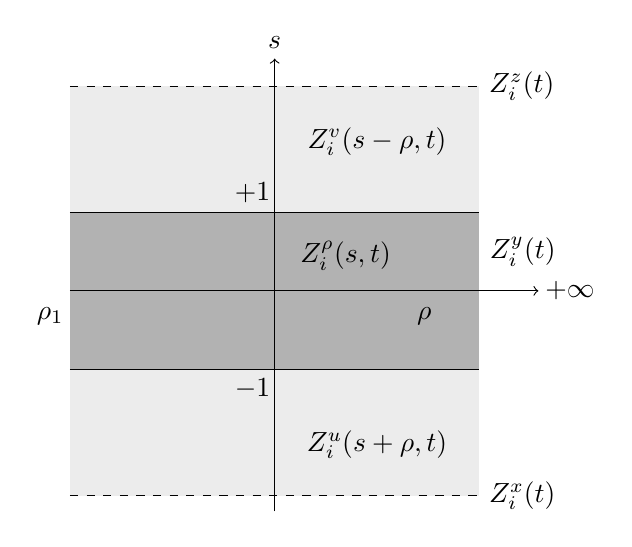
\begin{tikzpicture}[scale=1.0]
\fill[gray!15] (-2.6,1) rectangle (2.6,2.6);
\fill[gray!60] (-2.6,-1) rectangle (2.6,1);
\fill[gray!15] (-2.6,-2.6) rectangle (2.6,-1);
\draw (-2.6,1) -- (2.6,1);
\draw (-2.6,-1) -- (2.6,-1);
\draw[->] (0,-2.8) -- (0,2.95) node[above] {$s$};
\draw[->] (-2.6,0) -- (3.35,0);
\node at (3.75,0) {$+\infty$};
\node at (-2.85,-0.32) {$\rho_{1}$};
\node at (1.9,-0.32) {$\rho$};
\node at (-0.28,1.24) {$+1$};
\node at (-0.28,-1.24) {$-1$};
\node at (1.3,1.9) {$Z_{i}^{v}(s-\rho,t)$};
\node at (0.9,0.45) {$Z_{i}^{\rho}(s,t)$};
\node at (1.3,-1.95) {$Z_{i}^{u}(s+\rho,t)$};
\draw[dashed] (-2.6,2.6) -- (2.6,2.6) node[right] {$Z_{i}^{z}(t)$};
\draw[dashed] (-2.6,-2.6) -- (2.6,-2.6) node[right] {$Z_{i}^{x}(t)$};
\node at (3.15,0.5) {$Z_{i}^{y}(t)$};
\end{tikzpicture}
\caption{}
\label{fig:trivializations-w-rho}
\end{figure}

我们还没有完全做完：我们还需要 $w_{\rho}$ 的某个邻域内的\trTrivialization。对每个 $\rho$、每个 $s$ 与 $t$，以及对每个范数小于\trInjectivityRadius{}的切向量 $\xi\in T_{w_{\rho}(s,t)}W$，我们用\textbf{\trParallelTransport}（parallel transport；必要时参见\cref{sec:riemannian-metrics-exp}）来构造 $T_{\exp_{w_{\rho}(s,t)}(\xi)}W$ 的一个\trOrthonormal{}（但不必是\trUnitary{}的）基，我们把它记作 $(Z_{i}^{\rho,\xi}(s,t))_{i=1,\dots,2n}$。

\par\nopagebreak
\textbf{$\scr{F}_{\rho}$ 的定义。}\nopagebreak

对每个 $\rho\ge\rho_{0}$，我们定义一个算子
\[
\begin{array}{c}
W^{1,p}(\RR\times S^{1};\RR^{2n})\xrightarrow{\ \ \scr{F}_{\rho}\ \ }L^{p}(\RR\times S^{1};\RR^{2n})\\[8pt]
(y_{1},\dots,y_{2n})\longmapsto\Bigl[\Bigl(\frac{\partial}{\partial s}+J\frac{\partial}{\partial t}+\operatorname{grad}H_{t}\Bigr)\bigl(\exp_{w_{\rho}}\sum y_{i}Z_{i}^{\rho}\bigr)\Bigr]_{Z_{i}}\text{，}
\end{array}
\]
这个公式中的结果在基 $Z_{i}^{\rho,\sum y_{i}Z_{i}^{\rho}}$ 中展开，并且我们要注意，它并不定义一个\emph{线性}算子。映射 $\scr{F}_{\rho}$ 不是别的，正是
\[
\scr{F}_{\rho}=\scr{F}\circ\exp_{w_{\rho}}
\]
写在诸基 $Z_{i}$ 之下的样子。

\begin{remark}\label{thm:frho-well-defined}
映射 $\scr{F}_{\rho}$ 在球
\[
B(0,r_{0}/K)\subset W^{1,p}(\RR\times S^{1};\RR^{2n})
\]
中的诸向量 $(y_{1},\dots,y_{2n})$ 上是\trWellDefined{}的，其中 $r_{0}$ 选得小于 $W$ 上\trMetric{}的\trInjectivityRadius，而 $K$ 是 $W^{1,p}$ 到 $L^{\infty}$ 中的\trEmbedding{}的范数（使用\cref{sec:banach-manifold-p1p}中的记号——我们正是用那些记号来定义 $\scr{P}(x,y)$ 上的\trBanachManifold{}结构的）。

我们显然有 $\scr{F}_{\rho}(0)=\bigl[\scr{F}(w_{\rho})\bigr]_{Z_{i}^{\rho}}$。此外，由于 $u$ 与 $v$ 是\trFloerEquation{}的解，我们有
\[
\scr{F}(w_{\rho})=\frac{\partial w_{\rho}}{\partial s}+J\frac{\partial w_{\rho}}{\partial t}+\operatorname{grad}_{w_{\rho}}H_{t}=0\qquad\text{对 }|s|\ge 1\text{。}
\]
在 $[-1,1]$ 上，$w_{\rho}(s,t)$ 一致地（按 $\cC^{\infty}$ \trTopology）趋于 $y(t)$。于是，由于 $\scr{F}(y)=0$，当 $\rho$ 趋于 $+\infty$ 时，$\scr{F}(w_{\rho})$ 趋于 $0$，无论按 $\cC^{\infty}$ \trTopology{}还是按 $L^{p}$ \trTopology{}皆然。
\end{remark}

\par\nopagebreak
\textbf{\trNewton--\trPicard{}方法，总体思路。}\nopagebreak

我们要寻找一个 $\gamma=(\gamma_{1},\dots,\gamma_{2n})$，它是方程 $\scr{F}_{\rho}(\gamma)=0$ 的一个解。我们刚刚注意到，即便 $\scr{F}_{\rho}(0)=0$ 并不成立，原点 $0$ 也是该方程的一个“几乎”的解。我们将利用这个\trApproximateSolution{}作为出发点，借助\trNewton--\trPicard{}方法来构造一个真正的解。

就函数 $f\colon\RR\longrightarrow\RR$ 的情形而言，我们知道，这使我们能够从一个\trApproximateSolution $x_{0}$ 出发，把 $f$ 的一个零点 $\alpha$ 求成递归序列
\[
x_{n+1}=x_{n}-\frac{f(x_{n})}{f'(x_{n})}
\]
的极限。一个变体是把 $\alpha$ 求成序列
\[
x_{n+1}=x_{n}-\frac{f(x_{n})}{f'(x_{0})}
\]
的极限，其优点是只用到导数的一个值，而我们在这里对 $\scr{F}_{\rho}$ 要用的正是这个变体。这两种方法都表示在\cref{fig:newton-picard}之中。

\begin{figure}[htbp]
\centering
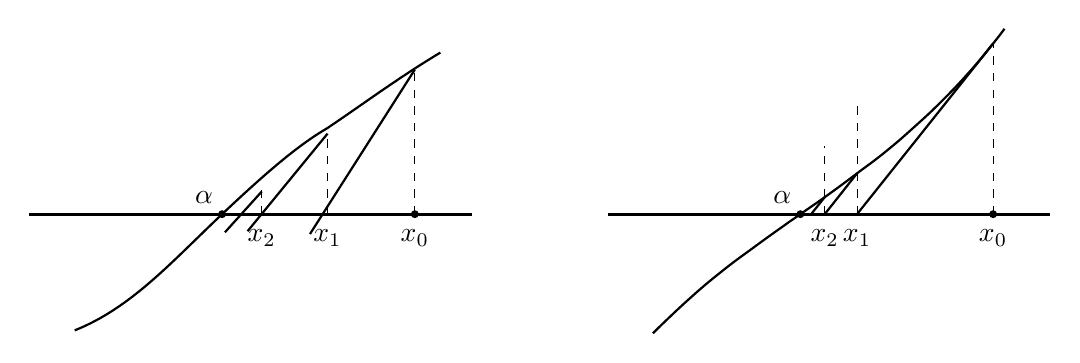
\begin{tikzpicture}[scale=0.72]
\begin{scope}
\draw[very thick] (-3.4,0) -- (4.4,0);
\draw[thick] (-2.6,-2.05) .. controls (-1.6,-1.65) and (-0.9,-0.85) .. (0,0)
      .. controls (0.9,0.85) and (1.4,1.25) .. (1.86,1.52)
      .. controls (2.5,1.95) and (3.1,2.4) .. (3.85,2.85);
\fill (0,0) circle (0.07);
\node at (-0.32,0.3) {$\alpha$};
\fill (3.4,0) circle (0.07);
\node at (3.4,-0.42) {$x_{0}$};
\node at (1.86,-0.42) {$x_{1}$};
\node at (0.7,-0.42) {$x_{2}$};
\draw[dashed] (3.4,0) -- (3.4,2.55);
\draw[dashed] (1.86,0) -- (1.86,1.4);
\draw[dashed] (0.7,0) -- (0.7,0.42);
\draw[thick] (3.4,2.55) -- (1.55,-0.35);
\draw[thick] (1.86,1.42) -- (0.45,-0.3);
\draw[thick] (0.7,0.4) -- (0.05,-0.32);
\end{scope}
\begin{scope}[xshift=10.2cm]
\draw[very thick] (-3.4,0) -- (4.4,0);
\draw[thick] plot[smooth, tension=0.8] coordinates {(-2.6,-2.1) (-2.0,-1.53) (-1.4,-1.02) (-0.8,-0.57) (-0.3,-0.21) (0,0) (0.5,0.35) (1.0,0.72) (1.5,1.1) (2.0,1.53) (2.5,2.0) (3.0,2.53) (3.4,3.01) (3.6,3.27)};
\fill (0,0) circle (0.07);
\node at (-0.32,0.3) {$\alpha$};
\fill (3.4,0) circle (0.07);
\node at (3.4,-0.42) {$x_{0}$};
\node at (1.0,-0.42) {$x_{1}$};
\node at (0.43,-0.42) {$x_{2}$};
\draw[dashed] (3.4,0) -- (3.4,3.01);
\draw[dashed] (1.0,0) -- (1.0,2.0);
\draw[dashed] (0.43,0) -- (0.43,1.2);
\draw[thick] (3.4,3.01) -- (1.0,0);
\draw[thick] (1.0,0.72) -- (0.43,0);
\draw[thick] (0.43,0.3) -- (0.19,0);
\end{scope}
\end{tikzpicture}
\caption{}
\label{fig:newton-picard}
\end{figure}

\textbf{$\scr{F}_{\rho}$ 的\trLinearization。}

现在我们来确定在\trNewton--\trPicard{}方法中扮演导数 $f'(x_{0})$ 这一角色的将是什么。我们让 $L_{\rho}$ 表示算子 $\scr{F}_{\rho}$ 在 $0$ 处的\trLinearization{} $(d\scr{F}_{\rho})_{0}$：
\[
L_{\rho}\colon W^{1,p}(\RR\times S^{1};\RR^{2n})\longrightarrow L^{p}(\RR\times S^{1};\RR^{2n})\text{。}
\]

\begin{proposition}\label{thm:lrho-fredholm-index2}
算子 $L_{\rho}$ 是一个\trIndex{}为 $2$ 的\trFredholmOperator。
\end{proposition}

\begin{proof}
我们在前一章中已经注意到（\cref{thm:chart-notation}），$\scr{F}$ 的\trDifferential{}对每个 $u$（而不仅仅是\trFloerEquation{}的那些解）都具有形式
\[
(d\scr{F})_{u}=\bar{\partial}+S(s,t)
\]
于是在我们的\trTrivialization{}中，我们有
\[
L_{\rho}(Y)=\frac{\partial Y}{\partial s}+J_{0}\frac{\partial Y}{\partial t}+S_{\rho}(s,t)Y
\]
其中一个映射
\[
S_{\rho}\colon\RR\times S^{1}\longrightarrow\mathrm{M}_{2n}(\RR)\text{。}
\]
由于我们已经把沿 $w_{\rho}$ 的\trTrivialization{}选取得与沿 $u$ 和 $v$ 的那些\trCompatible，故有
\[
S_{\rho}(s,t)=
\begin{cases}
S^{u}(s+\rho,t) & \text{对 }s\le-1\\
S^{v}(s-\rho,t) & \text{对 }s\ge 1\text{，}
\end{cases}
\]
其中 $S^{u}$ 与 $S^{v}$ 分别是 $\scr{F}$ 沿 $u$ 与 $v$ 在\trTrivialization{} $Z_{i}^{u}$ 与 $Z_{i}^{v}$ 中的\trLinearization{}所对应的那些矩阵。因此，特别地，当 $s$ 趋于 $\pm\infty$ 时，$S_{\rho}$ 趋于由\trCriticalPoint{} $x$ 与 $z$ 所定义的那两条\trSymmetricMatrix{}路径：\footnote{译注：原书此处印作“当 $\rho$ 趋于无穷时”；按紧随其后的极限式 $\lim_{s\to-\infty}S_{\rho}(s,t)=S^{x}(t)$、$\lim_{s\to+\infty}S_{\rho}(s,t)=S^{z}(t)$，以及 $S_{\rho}$ 的分段定义（$s\le-1$ 与 $s\ge1$ 两端分别与 $S^{u}$、$S^{v}$ 相合），趋于这两条路径的自变元是 $s$ 而非 $\rho$，此处径改。——译者注}
\[
\lim_{s\to-\infty}S_{\rho}(s,t)=S^{x}(t)\qquad\text{以及}\qquad\lim_{s\to+\infty}S_{\rho}(s,t)=S^{z}(t)\text{。}
\]
现在我们只需应用前一章的那些结果（即\cref{thm:fredholm-operator-L}与\cref{thm:index-maslov-difference}）：$L_{\rho}$ 是一个\trIndex{}为 $\mu(x)-\mu(z)=2$ 的\trFredholmOperator。
\end{proof}

\textbf{构造 $\psi$ 的思路。}

在我们的情形里，在\trNewton--\trPicard{}方法所用的那个递归序列的定义公式中，项 $1/f'(x_{0})$ 对应于\trLinearization{}后的映射 $L_{\rho}$ 的一个逆。$L_{\rho}$ 的\trIndex{}为 $2$ 这一事实使它不可能\trInvertible。我们将证明，$\operatorname{Ker}L_{\rho}$ 在 $W^{1,p}(\RR\times S^{1};\RR^{2n})$ 中存在一个\trClosed{}\trComplement{} $W_{\rho}^{\perp}$，使得 $L_{\rho}|_{W_{\rho}^{\perp}}$ 是\trInvertible{}的（换句话说，$L_{\rho}$ 在 $W_{\rho}^{\perp}$ 上存在一个右逆）。我们将从\trApproximateSolution $0$ 出发应用\trNewton--\trPicard{}方法，以求得 $\scr{F}_{\rho}(\gamma)=0$ 的一个解。

\begin{figure}[htbp]
\centering
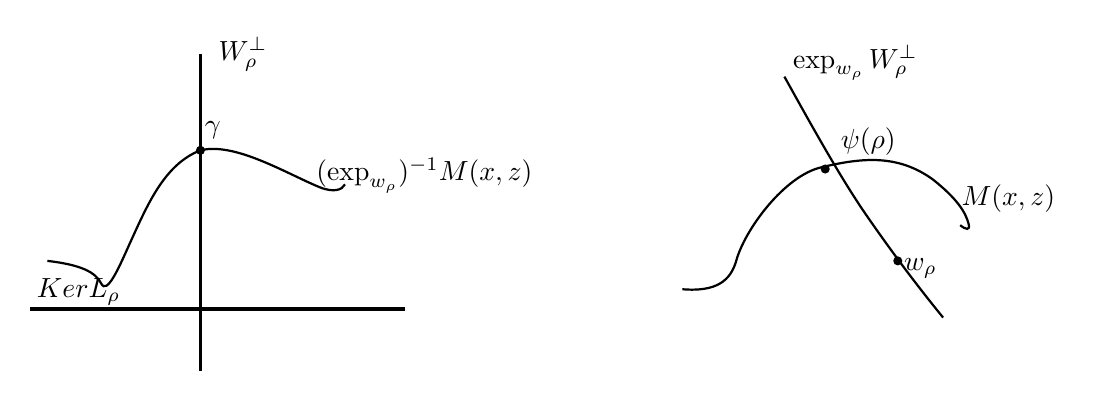
\begin{tikzpicture}[scale=0.72]
\begin{scope}
\draw[thick] (0.4,-3.1) -- (0.4,2.5);
\draw[very thick] (-2.6,-2.0) -- (4.0,-2.0);
\node at (1.15,2.5) {$W_{\rho}^{\perp}$};
\node at (-1.75,-1.7) {$\operatorname{Ker}L_{\rho}$};
\draw[thick] (-2.3,-1.15) .. controls (-1.7,-1.22) and (-1.45,-1.35) .. (-1.35,-1.55)
      .. controls (-1.25,-1.75) and (-1.05,-1.3) .. (-0.85,-0.85)
      .. controls (-0.55,-0.2) and (-0.25,0.55) .. (0.4,0.8)
      .. controls (1.0,0.95) and (1.9,0.4) .. (2.5,0.15)
      .. controls (2.75,0.05) and (2.9,0.1) .. (2.95,0.2);
\fill (0.4,0.8) circle (0.08);
\node at (0.62,1.15) {$\gamma$};
\node at (4.35,0.35) {$({\exp_{w_{\rho}}})^{-1}\scr{M}(x,z)$};
\end{scope}
\begin{scope}[xshift=10.6cm]
\draw[thick] (0.1,2.1) .. controls (0.6,1.2) and (1.1,0.3) .. (1.55,-0.35)
      .. controls (2.0,-1.0) and (2.45,-1.6) .. (2.9,-2.15);
\node at (1.35,2.35) {$\exp_{w_{\rho}}W_{\rho}^{\perp}$};
\draw[thick] (-1.7,-1.65) .. controls (-1.1,-1.7) and (-0.85,-1.5) .. (-0.75,-1.15)
      .. controls (-0.6,-0.6) and (0.1,0.35) .. (0.75,0.5)
      .. controls (1.5,0.68) and (2.1,0.72) .. (2.7,0.3)
      .. controls (3.15,-0.05) and (3.3,-0.3) .. (3.35,-0.5)
      .. controls (3.38,-0.62) and (3.3,-0.6) .. (3.2,-0.52);
\fill (0.82,0.47) circle (0.08);
\fill (2.1,-1.15) circle (0.08);
\node at (1.58,0.95) {$\psi(\rho)$};
\node at (2.5,-1.28) {$w_{\rho}$};
\node at (4.05,-0.05) {$\scr{M}(x,z)$};
\end{scope}
\end{tikzpicture}
\caption{}
\label{fig:construction-idea}
\end{figure}

我们需要使用这样一个子空间 $W_{\rho}^{\perp}$，这一点并不令人惊讶：我们知道 $\scr{M}(x,z)$ 是一个维数为 $2$ 的\trManifold；因此对每个 $\rho$，我们要寻找的乃是 $(\exp_{w_{\rho}})^{-1}\scr{M}(x,z)$ 的一个元素 $\gamma$，后者是 $T_{w_{\rho}}\scr{P}(x,z)$ 的一个维数为 $2$ 的\trSubmanifold。把这个\trSubmanifold{}与一个余维数为 $2$ 的子空间——也就是我们的 $W_{\rho}^{\perp}$——相交来确定这样的一个 $\gamma$，看起来是自然的（我们的确将会证明 $\dim\operatorname{Ker}L_{\rho}=2$）。\cref{fig:construction-idea}对此作了示意。

于是，我们将把路径 $\psi(\rho)$ 求成 $\scr{M}(x,z)$ 与空间
\[
\bigl\{\exp_{w_{\rho}}W_{\rho}^{\perp}\ \bigm|\ \rho\ge\rho_{0}\bigr\}
\]
在 $\scr{P}(x,z)$ 中的交集。这个子空间的余维数为 $1$；它是\trFiberBundle{} $W^{\perp}$ 的像，后者由诸 $W_{\rho}^{\perp}$（在 $w_{\rho}$ 上的）组成，是 $w^{\star}T\scr{P}(x,z)$ 的一个余维数为 $2$ 的\textbf{\trSubbundle}（subbundle）。\cref{fig:w-perp-leaves}对此作了示意。

\begin{figure}[htbp]
\centering
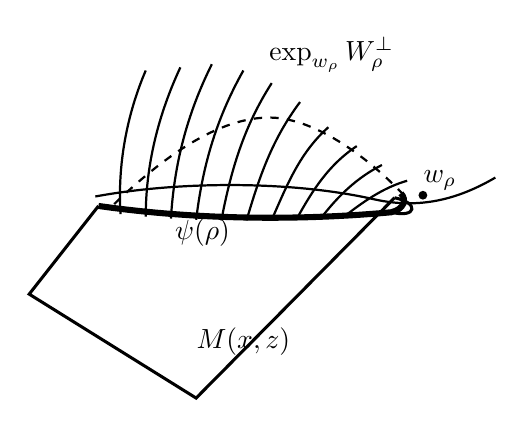
\begin{tikzpicture}[scale=0.8]
\draw[line width=2.2pt] (0.2,1.15)
      .. controls (1.6,0.95) and (3.2,0.9) .. (4.85,1.05)
      .. controls (5.05,1.1) and (5.1,1.25) .. (5.0,1.35);
\draw[line width=1.1pt] (0.2,1.15) -- (-0.9,-0.25) -- (1.75,-1.9) -- (4.9,1.28);
\draw[line width=1.1pt] (4.85,1.05) .. controls (5.25,0.95) and (5.3,1.2) .. (4.9,1.28);
\node at (2.5,-1.0) {$\scr{M}(x,z)$};
\node at (1.85,0.72) {$\psi(\rho)$};
\draw[thick] (0.55,1.02) .. controls (0.5,1.8) and (0.65,2.6) .. (0.95,3.3);
\draw[thick] (0.95,0.98) .. controls (0.95,1.8) and (1.15,2.6) .. (1.5,3.35);
\draw[thick] (1.35,0.95) .. controls (1.4,1.8) and (1.6,2.6) .. (2.0,3.4);
\draw[thick] (1.75,0.93) .. controls (1.85,1.75) and (2.05,2.5) .. (2.5,3.3);
\draw[thick] (2.15,0.92) .. controls (2.3,1.7) and (2.5,2.4) .. (2.95,3.1);
\draw[thick] (2.55,0.92) .. controls (2.75,1.6) and (2.95,2.2) .. (3.4,2.8);
\draw[thick] (2.95,0.93) .. controls (3.2,1.5) and (3.4,2.0) .. (3.85,2.4);
\draw[thick] (3.35,0.95) .. controls (3.6,1.4) and (3.85,1.8) .. (4.3,2.1);
\draw[thick] (3.75,0.98) .. controls (4.0,1.3) and (4.3,1.6) .. (4.7,1.8);
\draw[thick] (4.15,1.02) .. controls (4.45,1.25) and (4.75,1.45) .. (5.1,1.55);
\draw[thick] (0.15,1.3) .. controls (1.5,1.55) and (3.3,1.55) .. (4.6,1.25)
      .. controls (5.3,1.1) and (5.9,1.25) .. (6.5,1.6);
\draw[dashed, thick] (0.45,1.18) .. controls (1.3,2.0) and (2.2,2.6) .. (3.0,2.55)
      .. controls (3.7,2.5) and (4.5,1.9) .. (5.05,1.32);
\node at (3.9,3.55) {$\exp_{w_{\rho}}W_{\rho}^{\perp}$};
\fill (5.35,1.32) circle (0.07);
\node at (5.62,1.55) {$w_{\rho}$};
\end{tikzpicture}
\caption{}
\label{fig:w-perp-leaves}
\end{figure}

\textbf{（抽象的）\trNewton--\trPicard{}方法。}

下面就是我们将要使用的精确陈述。

\begin{lemma}\label{thm:abstract-newton-picard}
设 $X$ 与 $Y$ 是两个\trBanachSpace，并设 $F\colon X\longrightarrow Y$ 是一个连续映射。我们写
\[
F(x)=F(0)+L(x)+N(x)\text{，}
\]
其中 $L(x)=(dF)_{0}(x)$，并且我们假设存在一个连续线性的 $G\colon Y\longrightarrow X$\footnote{译注：原书仅设 $G$ 连续；但本条证明反复使用 $G$ 的可加性，例如 $\varphi(x)=-G\bigl(F(0)+N(x)\bigr)=-GF(0)-GN(x)$ 与 $\|\varphi(x)-\varphi(y)\|=\|GN(x)-GN(y)\|$ 两条都以 $G(a+b)=G(a)+G(b)$ 为前提（仅有连续性时有显式反例），故 $G$ 须设为连续线性映射，此处径改补“线性”。——译者注}，使得：
\begin{enumerate}[label=(\arabic*)]
\item $L\circ G=\mathrm{Id}$。
\item $\|GN(x)-GN(y)\|\le C\left(\|x\|+\|y\|\right)\|x-y\|$ 对所有的 $x$、$y\in B(0,r)$ 成立。
\item $\|GF(0)\|\le\varepsilon/2$，其中 $\varepsilon=\min\left(r,1/5C\right)$。
\end{enumerate}
那么，存在一个唯一的 $\alpha\in\operatorname{Im}(G)\cap B(0,\varepsilon)$ 使得 $F(\alpha)=0$。此外，我们有 $\|\alpha\|\le 2\|GF(0)\|$。
\end{lemma}

\begin{proof}
本着经典的\trNewton--\trPicard{}方法，我们如下定义 $\varphi\colon B(0,\varepsilon)\longrightarrow\operatorname{Im}(G)$：
\[
\varphi(x)=G\bigl(L(x)-F(x)\bigr)=-G\bigl(F(0)+N(x)\bigr)\text{。}
\]
注意到
\[
L\varphi(x)=L(x)-F(x)\text{。}
\]
于是，若 $\varphi(x)=x$，则 $F(x)=0$。反之，若 $F(x)=0$ 且 $x=G(y)$，则
\[
\varphi(x)=GL(x)=GLG(y)=G(y)=x\text{。}
\]
因此我们将证明，$\varphi$ 在 $B(0,\varepsilon)$ 中有唯一的一个\trFixedPoint。

首先，$\varphi$ 把半径为 $\varepsilon$ 的球映入其自身：若 $\|x\|\le\varepsilon$，则
\[
\begin{aligned}
\|\varphi(x)\|=\bigl\|G\bigl(F(0)+N(x)\bigr)\bigr\|&\le\|GF(0)\|+\|GN(x)\|\\
&\le\frac{\varepsilon}{2}+C\|x\|^{2}\\
&\le\frac{\varepsilon}{2}+C\varepsilon^{2}\\
&\le\frac{\varepsilon}{2}+\frac{\varepsilon}{5}<\varepsilon\text{，}
\end{aligned}
\]
在这一串不等式中，我们用到了性质 (2) 与性质 (3)，以及 $N(0)=0$ 这一事实。

其次，若 $x$ 与 $y$ 是球 $B(0,\varepsilon)$ 中的两点，则
\[
\begin{aligned}
\|\varphi(x)-\varphi(y)\|=\|GN(x)-GN(y)\|&\le C\left(\|x\|+\|y\|\right)\|x-y\|\\
&\le 2C\varepsilon\,\|x-y\|\\
&\le\frac{2}{5}\,\|x-y\|\le\frac{1}{2}\,\|x-y\|\text{。}
\end{aligned}
\]
于是，由
\[
x_{0}=0\qquad\text{以及}\qquad x_{n+1}=\varphi(x_{n})
\]
所定义的序列是一个\trCauchy{}序列，从而它\trConvergence{}于一个极限 $\alpha$，后者是 $\varphi$ 的一个\trFixedPoint，并且由于我们刚刚证明的那条不等式，它是唯一的\trFixedPoint。

最后，作为收尾，我们来证明这条引理所陈述的那条不等式。我们有
\[
\frac{1}{2}\,\|\alpha\|=\frac{1}{2}\,\|\alpha-0\|\ge\|\varphi(\alpha)-\varphi(0)\|=\|\alpha-\varphi(0)\|\ge\|\alpha\|-\|\varphi(0)\|\text{。}
\]
由此推出
\[
\|\alpha\|\le 2\,\|\varphi(0)\|=2\,\|GF(0)\|\text{。}
\]
\end{proof}

\textbf{引理~9.4.4~的应用。}

我们将把这条引理应用于映射
\[
\scr{F}_{\rho}\colon W^{1,p}(\RR\times S^{1};\RR^{2n})\longrightarrow L^{p}(\RR\times S^{1};\RR^{2n})\text{。}
\]
因此我们需要确定 $L_{\rho}$ 在 $0$ 处的\trDifferential{}的一个右逆 $G_{\rho}$，并验证这个 $G_{\rho}$ 满足引理的各个条件。正如我们已经说过的，我们将借助一个子空间 $W_{\rho}^{\perp}$ 来得到 $G_{\rho}$，于是我们先来定义后者。

在\trTrivialization{} $Z_{i}^{u}$ 与 $Z_{i}^{v}$ 中，我们把诸\trDifferential{} $(d\scr{F})_{u}$ 与 $(d\scr{F})_{v}$ 分别记作 $L^{u}$ 与 $L^{v}$；经由这些\trTrivialization，我们考虑
\[
\operatorname{Ker}L^{u}\subset T_{u}\scr{P}(x,y)\qquad\text{以及}\qquad\operatorname{Ker}L^{v}\subset T_{v}\scr{P}(y,z)\text{。}
\]
我们定义 $W_{\rho}$ 为这些子空间的“$\#_{\rho}$ 和”：
\[
W_{\rho}=\bigl\{\alpha\#_{\rho}\beta\ \bigm|\ \alpha\in\operatorname{Ker}L^{u}\text{，}\ \beta\in\operatorname{Ker}L^{v}\bigr\}\text{。}
\]
然后我们定义 $W_{\rho}^{\perp}$ 为它的\trOrthogonal{}补，也就是说
\[
\begin{aligned}
W_{\rho}^{\perp}={}&\Bigl\{Y\in W^{1,p}(\RR\times S^{1};\RR^{2n})\ \Bigm|\\
&\int_{\RR\times S^{1}}\langle Y,\alpha\#_{\rho}\beta\rangle\,ds\,dt=0\ \text{对所有的 }\alpha\in\operatorname{Ker}L^{u}\text{，}\beta\in\operatorname{Ker}L^{v}\Bigr\}\text{，}
\end{aligned}
\]
（仍然使用\trFrame{} $(Z_{i}^{\rho})_{i=1,\dots,2n}$，以便把 $\alpha\#_{\rho}\beta$ 视为 $W^{1,p}(\RR\times S^{1};\RR^{2n})$ 的一个元素）。

\begin{remark}\label{thm:remarks-w-perp}
\begin{enumerate}[label=(\arabic*)]
\item \trFloerEquation{}的两个解 $u$ 与 $v$ 连接着具有相继\trIndex{}的\trCriticalPoint。由于偶对 $(H,J)$ 是\trRegular{}的，因此我们知道 $L^{u}$ 与 $L^{v}$ 都是\trSurjective{}的。由于它们的\trFredholm{}\trIndex{}都是 $1$，故 $L^{u}$ 与 $L^{v}$ 的\trKernel{}的维数都是 $1$。由\cref{thm:df-kernel-nontrivial}，我们于是可以断言
\[
\operatorname{Ker}L^{u}=\RR\cdot\frac{\partial u}{\partial s}\qquad\text{以及}\qquad\operatorname{Ker}L^{v}=\RR\cdot\frac{\partial v}{\partial s}
\]
（这里隐含地用到了\trFrame{} $(Z_{i}^{u})$、$(Z_{i}^{v})$）。
\item 由于由\trExponentialDecay{}（\cref{sec:exponential-decay}）我们有
\[
\sup\Bigl(\Bigl|\frac{\partial u}{\partial s}\Bigr|,\Bigl|\frac{\partial v}{\partial s}\Bigr|\Bigr)\le Ke^{-\delta|s|}\text{，}
\]
我们知道向量 $\partial u/\partial s$ 与 $\partial v/\partial s$ 都属于 $L^{q}$（对每个 $q\ge 1$），从而
\[
\forall Y\in W^{1,p}(\RR\times S^{1};\RR^{2n})\text{，}\ \forall\alpha\in\operatorname{Ker}L^{u}\text{，}\ \forall\beta\in\operatorname{Ker}L^{v}\text{，}\quad\langle Y,\alpha\#_{\rho}\beta\rangle\in L^{1}\text{。}
\]
\item 空间 $W^{1,p}(\RR\times S^{1};\RR^{2n})$ 是 $W_{\rho}$ 与 $W_{\rho}^{\perp}$ 的\trDirectSum。这是一个简单而且相当一般的事实，我们可以把它陈述成一条引理。

\begin{lemma}\label{thm:direct-sum-splitting}
设 $1/p+1/q=1$。设 $E$ 是 $W^{1,p}\cap L^{q}$ 的一个有限维子空间。令
\[
E^{\perp}=\Bigl\{Y\in W^{1,p}\ \Bigm|\ \int\langle Y,X\rangle\,ds\,dt=0\ \text{对每个 }X\in E\Bigr\}\text{。}
\]
那么 $W^{1,p}=E\oplus E^{\perp}$。
\end{lemma}

\begin{proof}
的确，这两个子空间显然只在 $0$ 处相交。其次，由\trHoelder{}不等式，由于 $E\subset L^{p}\cap L^{q}$，我们有 $E\subset L^{2}$。于是只需选取 $E$ 的一个\trOrthonormal{}基 $\{e_{1},\dots,e_{r}\}$。$W^{1,p}$ 的每个元素 $Z$ 都满足
\[
Z-\langle e_{1},Z\rangle e_{1}-\dots-\langle e_{r},Z\rangle e_{r}\in E^{\perp}\text{，}
\]
这就给出了所期待的结果。
\end{proof}

由于 $W_{\rho}$ 是二维空间 $\operatorname{Ker}L^{u}\times\operatorname{Ker}L^{v}$ 在线性映射 $\#_{\rho}$ 下的\trImage，我们知道 $\dim W_{\rho}\le 2$，从而可以应用\cref{thm:direct-sum-splitting}。
\end{enumerate}
\end{remark}

下面的这条命题是重要的。它使我们能够定义 $G_{\rho}$ 并验证引理的各个条件。

\begin{proposition}\label{thm:lrho-lower-bound}
存在一个常数 $C>0$，使得对 $\rho\ge\rho_{0}$，我们有
\[
\forall Y\in W_{\rho}^{\perp}\text{，}\quad\|L_{\rho}(Y)\|_{L^{p}}\ge C\,\|Y\|_{W^{1,p}}\text{。}
\]
\end{proposition}

我们先来给出这条命题的一系列推论。我们假设 $\rho\ge\rho_{0}$。

\begin{enumerate}[label=(\arabic*)]
\item 首先，我们显然有 $\operatorname{Ker}L_{\rho}\cap W_{\rho}^{\perp}=0$。
\item 映射 $L_{\rho}$ 是\trSurjective{}的，并且 $\dim\operatorname{Ker}L_{\rho}=\dim W_{\rho}=2$。事实上，我们总有
\[
\dim\operatorname{Ker}L_{\rho}\ge\operatorname{Ind}(L_{\rho})=2
\]
以及
\[
\operatorname{codim}W_{\rho}^{\perp}=\dim W_{\rho}\le\dim\left(\operatorname{Ker}L^{u}\times\operatorname{Ker}L^{v}\right)=2
\]
而第一条性质把这两个不等式都变成了等式。因此我们有
\[
W^{1,p}(\RR\times S^{1};\RR^{2n})=\operatorname{Ker}L_{\rho}\oplus W_{\rho}^{\perp}\text{。}
\]

直观上，我们可以说：当 $\rho$ 充分大时，$(d\scr{F})_{u\#_{\rho}v}$ 的\trKernel{}与 $\operatorname{Ker}(d\scr{F})_{u}\#_{\rho}\operatorname{Ker}(d\scr{F})_{v}$ 相距不远。
\item 从而，
\[
L_{\rho}\colon W_{\rho}^{\perp}\cong W^{1,p}(\RR\times S^{1};\RR^{2n})/\operatorname{Ker}L_{\rho}\longrightarrow L^{p}(\RR\times S^{1};\RR^{2n})=\operatorname{Im}L_{\rho}
\]
是\trBijective{}的。我们令
\[
G_{\rho}=L_{\rho}^{-1}\colon L^{p}(\RR\times S^{1};\RR^{2n})\longrightarrow W_{\rho}^{\perp}\text{。}
\]
\item 这个映射 $G_{\rho}$ 是连续的，因为这条命题断言
\[
\|G_{\rho}(Y)\|_{W^{1,p}}\le\frac{1}{C}\,\|L_{\rho}G_{\rho}(Y)\|_{L^{p}}=\frac{1}{C}\,\|Y\|_{L^{p}}\text{。}
\]
\end{enumerate}

\cref{thm:abstract-newton-picard}的条件 (2) 与条件 (3) 也是\cref{thm:lrho-lower-bound}的推论：

\begin{enumerate}[label=(\arabic*)]
\item 首先，我们来验证\cref{thm:abstract-newton-picard}的条件 (2)（在记号中把 $\rho$ 略去不写）。我们有
\[
\|GNx-GNy\|\le C^{-1}\|N(x)-N(y)\|\le C^{-1}\sup_{z\in[x,y]}\|(dN)_{z}\|\,\|x-y\|
\]
（由中值定理）。在线段 $[x,y]$ 上，$\|(dN)_{z}\|$ 以 $K\|z\|$ 为界，其中 $K$ 不依赖于 $\rho$、$x$ 与 $y$，这由\cref{thm:dn-op-estimate}——在\cref{sec:two-lemmas-df}中所证明的技术性引理之一——给出：
\[
\|(dN)_{z}\|\le K\|z\|
\]
因为
\[
(dN)_{z}=(d\scr{F})_{z}-(d\scr{F})_{0}\text{。}
\]
由此推出
\[
\begin{aligned}
\|GNx-GNy\|&\le C^{-1}\|N(x)-N(y)\|\\
&\le C^{-1}K\sup_{z\in[x,y]}\|z\|\,\|x-y\|\\
&\le C^{-1}K\left(\|x\|+\|y\|\right)\|x-y\|
\end{aligned}
\]
而条件 (2) 得到满足。\footnote{译注：原书此不等式链第二行的 $\sup$ 下标印作 $z\in[x,y])$，括号多出一枚；按其上一不等式（同一下标处）印作 $z\in[x,y]$，疑为排印衍文，此处径删。——译者注}

\begin{lemma}\label{thm:dn-op-estimate}
设 $r_{0}>0$。存在一个常数 $K>0$，使得对每个 $\rho\ge\rho_{0}$ 与每个 $Z\in\overline{B}(0,r_{0})\subset W^{1,p}(\RR\times S^{1};\RR^{2n})$，我们有
\[
\|(d\scr{F}_{\rho})_{Z}-(d\scr{F}_{\rho})_{0}\|^{\mathrm{op}}\le K\|Z\|_{W^{1,p}}\text{。}
\]
\end{lemma}

\item 最后，我们来验证\cref{thm:abstract-newton-picard}的条件 (3)。我们有
\[
\|G_{\rho}\scr{F}_{\rho}(0)\|\le C^{-1}\|\scr{F}_{\rho}(0)\|=C^{-1}\|\scr{F}(w_{\rho})\|\text{，}
\]
而当 $\rho$ 趋于无穷时它趋于 $0$，于是当 $\rho$ 充分大时，我们的确有 $\|G_{\rho}\scr{F}_{\rho}(0)\|\le\varepsilon/2$。现在我们可以应用\trNewton--\trPicard{}引理了。
\end{enumerate}

\begin{proof}[\cref{thm:lrho-lower-bound}的证明]
我们采用反证的推理方式。假设存在一列趋于无穷的 $(\rho_{n})$ 以及一列 $Y_{n}\in W_{\rho_{n}}^{\perp}$，使得
\[
\lim_{n\to+\infty}\frac{\|L_{\rho_{n}}Y_{n}\|_{L^{p}}}{\|Y_{n}\|_{W^{1,p}}}=0\text{。}
\]
通过规范化，我们可以（并且也确实）假设 $\|Y_{n}\|=1$。

\begin{lemma}\label{thm:yn-locally-small}
设 $K=[-a,a]\times S^{1}\subset\RR\times S^{1}$。那么
\[
\lim_{n\to+\infty}\|Y_{n}\|_{W^{1,p}(K)}=0\text{。}
\]
\end{lemma}

\begin{proof}
考虑算子
\[
D\colon W^{1,p}(\RR\times S^{1};\RR^{2n})\longrightarrow L^{p}(\RR\times S^{1};\RR^{2n})
\]
它由
\[
D(Y)=\frac{\partial Y}{\partial s}(s,t)+J_{0}\frac{\partial Y}{\partial t}(s,t)+S^{y}(t)\cdot Y(s,t)
\]
来定义，其中 $t\mapsto S^{y}(t)$ 是对应于沿\trLoop{} $y$ 所选取的\trTrivialization{}的那条\trSymmetricMatrix{}路径。正如我们已经知道的，\footnote{译注：原书此式第三项印作 $-(dJ)_{w_{\rho}}(Y)\,\frac{\partial w_{\rho}}{\partial t}$；把 $w_{\rho}$ 换成 $w_{\rho}+\varepsilon Y$ 后对 $\varepsilon$ 求导，$J$ 项的一阶展开为 $J\frac{\partial Y}{\partial t}+(dJ)_{w_{\rho}}(Y)\frac{\partial w_{\rho}}{\partial t}$，故第三项应为正号，此处径改。——译者注}
\[
(d\scr{F})_{w_{\rho}}(Y)=\frac{\partial Y}{\partial s}+J\frac{\partial Y}{\partial t}+(dJ)_{w_{\rho}}(Y)\frac{\partial w_{\rho}}{\partial t}+d\bigl(\operatorname{grad}_{w_{\rho}}H_{t}\bigr)(Y)\text{。}
\]
由于当 $\rho$ 趋于无穷时，$w_{\rho}$ 趋于 $y$（按 $\cC^{\infty}_{\mathrm{loc}}$ 的意义），这个算子的零阶部分趋于 $(d\scr{F})_{y}$ 的零阶部分。又由于我们选取诸\trTrivialization{}的方式使得 $Z_{i}^{\rho}(s,t)$ 趋于 $Z_{i}^{y}(t)$（仍按 $\cC^{\infty}_{\mathrm{loc}}$ 的意义），故有
\[
\lim_{\rho\to\infty}S_{\rho}(s,t)=S^{y}(t)\quad\text{按 }\cC^{\infty}_{\mathrm{loc}}\text{ 的意义。}
\]
令 $r_{n}=\rho_{n}/2$。我们选取一个\trPlateauFunction{} $\gamma$，它在 $|s|\le 1/2$ 时取值 $1$，在 $|s|\ge 1$ 时取值 $0$，并令 $\gamma_{n}(s)=\gamma(s/r_{n})$。

我们来证明 $D(\gamma_{n}Y_{n})$ 按 $L^{p}$ 范数趋于 $0$。事实上我们有
\[
\begin{aligned}
\|D(\gamma_{n}Y_{n})\|_{L^{p}}=\Bigl\|\gamma_{n}D(Y_{n})+\frac{1}{r_{n}}\dot{\gamma}\Bigl(\frac{s}{r_{n}}\Bigr)Y_{n}\Bigr\|_{L^{p}}&\le\frac{1}{r_{n}}\Bigl\|\dot{\gamma}\Bigl(\frac{s}{r_{n}}\Bigr)Y_{n}\Bigr\|_{L^{p}}+\|\gamma_{n}D(Y_{n})\|_{L^{p}}\\
&\le\frac{M}{r_{n}}\|Y_{n}\|_{L^{p}}+\|D(Y_{n})\|_{L^{p}([-r_{n},r_{n}]\times S^{1})}\text{，}
\end{aligned}
\]
其中 $M$ 是 $|\dot{\gamma}(s)|$ 在 $\RR$ 上的上界。由此推出
\[
\begin{aligned}
\|D(\gamma_{n}Y_{n})\|_{L^{p}}&\le\frac{M}{r_{n}}\|Y_{n}\|_{L^{p}}+\|(D-L_{\rho_{n}})Y_{n}\|_{L^{p}([-r_{n},r_{n}]\times S^{1})}\\
&\qquad\qquad+\|L_{\rho_{n}}(Y_{n})\|_{L^{p}([-r_{n},r_{n}]\times S^{1})}\\
&\le\frac{M}{r_{n}}\|Y_{n}\|_{L^{p}}+\|(S^{y}-S_{\rho_{n}})Y_{n}\|_{L^{p}([-r_{n},r_{n}]\times S^{1})}\\
&\qquad\qquad+\|L_{\rho_{n}}(Y_{n})\|_{L^{p}}\text{。}
\end{aligned}
\]
由于 $\|Y_{n}\|_{L^{p}}\le\|Y_{n}\|_{W^{1,p}}=1$，并且由于 $\|L_{\rho_{n}}(Y_{n})\|_{L^{p}}$ 趋于 $0$，这就给出
\[
\|D(\gamma_{n}Y_{n})\|_{L^{p}}\le\|(S^{y}-S_{\rho_{n}})Y_{n}\|_{L^{p}}+\tau_{n}
\]
对一个当 $n$ 趋于无穷时趋于 $0$ 的 $\tau_{n}\ge 0$。其次，注意到
\[
\begin{aligned}
\|(S^{y}-S_{\rho_{n}})Y_{n}\|_{L^{p}([-r_{n},r_{n}]\times S^{1})}&\le\sup_{(s,t)\in[-r_{n},r_{n}]\times S^{1}}\|S_{\rho_{n}}(s,t)-S^{y}(t)\|\,\|Y_{n}\|_{L^{p}}\\
&\le\sup_{(s,t)\in[-r_{n},r_{n}]\times S^{1}}\|S_{\rho_{n}}(s,t)-S^{y}(t)\|\text{。}
\end{aligned}
\]
对 $s\le-1$，我们有 $S_{\rho_{n}}(s,t)=S^{u}(s+\rho_{n},t)$；于是，$\|S_{\rho_{n}}(s,t)-S^{y}(t)\|$ 在 $(s,t)\in[-r_{n},-1]\times S^{1}$ 上的上确界就等于
\[
\sup_{(s,t)\in[-r_{n},-1]\times S^{1}}\bigl\|S^{u}(s+\rho_{n},t)-S^{y}(t)\bigr\|\text{，}
\]
也就是说，
\[
\sup_{(s,t)\in[r_{n},\rho_{n}-1]\times S^{1}}\bigl\|S^{u}(s,t)-S^{y}(t)\bigr\|\text{，}
\]
因而这个上确界趋于 $0$。同样地，对 $s\ge 1$，利用 $S_{\rho_{n}}(s,t)=S^{v}(s-\rho_{n},t)$ 这一事实，我们可以验证
\[
\lim_{n\to+\infty}\sup_{(s,t)\in[1,r_{n}]\times S^{1}}\|S_{\rho_{n}}(s,t)-S^{y}(t)\|=0\text{。}
\]
最后，我们有
\[
\lim_{n\to+\infty}\sup_{(s,t)\in[-1,1]\times S^{1}}\|S_{\rho_{n}}(s,t)-S^{y}(t)\|=0
\]
因为 $S_{\rho_{n}}(s,t)$ 按 $\cC^{\infty}_{\mathrm{loc}}$ 的意义趋于 $S^{y}(t)$。这样我们就证明了 $D(\gamma_{n}Y_{n})$ 按 $L^{p}$ 范数趋于 $0$，这就使我们得以结束引理的证明。

我们知道（参见\cref{thm:d-bijective-independent-s}，它处于“$\scr{F}$ 是一个\trFredholmOperator”这一事实的证明之中），$D\colon W^{1,p}(\RR\times S^{1};\RR^{2n})\longrightarrow L^{p}(\RR\times S^{1};\RR^{2n})$ 是\trInvertible{}的。由 $\|D(\gamma_{n}Y_{n})\|_{L^{p}}$ 趋于 $0$ 这一事实，我们推出 $\|\gamma_{n}Y_{n}\|_{W^{1,p}}$ 趋于 $0$，从而
\[
\lim_{n\to+\infty}\|Y_{n}\|_{W^{1,p}(K)}=0\text{，}
\]
这就结束了引理的证明。
\end{proof}

由于 $Y_{n}$ 的 $W^{1,p}$ 范数是 $1$，这条引理断言：它的\trSupport{}趋向于朝 $|s|\to+\infty$ 集中。

我们将利用当 $|s|$ 充分大时 $L_{\rho_{n}}$、$L^{u}$ 与 $L^{v}$ 之间的关系。

\begin{lemma}\label{thm:translated-subsequences}
设 $\beta^{\pm}$ 是用来构造\trApproximateSolution $w_{\rho}$ 的那两个函数。存在\trVectorField{} $Y\in\operatorname{Ker}L^{u}$ 与 $Z\in\operatorname{Ker}L^{v}$，使得在必要时抽取子序列之后，
\[
\beta^{-}(s-\rho_{n}+1)Y_{n}(s-\rho_{n},t)\quad\text{在 }W^{1,p}(\RR\times S^{1};\RR^{2n})\text{ 中趋于 }Y\text{，}
\]
并且
\[
\beta^{+}(s+\rho_{n}-1)Y_{n}(s+\rho_{n},t)\quad\text{在 }W^{1,p}(\RR\times S^{1};\RR^{2n})\text{ 中趋于 }Z\text{。}
\]
\end{lemma}

\begin{proof}
回顾一下，$\beta^{-}(s+1)=0$ 对 $s\ge-1$ 成立，这意味着 $\beta^{-}(s+1)Y_{n}(s,t)$ 的\trSupport{}含于 $]-\infty,-1]\times S^{1}$ 之中。由此可得
\[
\begin{aligned}
\bigl\|L^{u(s+\rho_{n},t)}\bigl(\beta^{-}(s+1)Y_{n}(s,t)\bigr)\bigr\|_{L^{p}}&=\bigl\|L_{\rho_{n}}\bigl(\beta^{-}(s+1)Y_{n}(s,t)\bigr)\bigr\|_{L^{p}}\\
&=\Bigl\|\dot{\beta}^{-}(s+1)Y_{n}(s,t)+\beta^{-}(s+1)L_{\rho_{n}}\bigl(Y_{n}(s,t)\bigr)\Bigr\|_{L^{p}}\\
&\le\sup\dot{\beta}^{-}\,\|Y_{n}\|_{L^{p}([-1,1]\times S^{1})}+\|L_{\rho_{n}}Y_{n}\|_{L^{p}}\text{，}
\end{aligned}
\]
由\cref{thm:yn-locally-small}，它趋于 $0$。\footnote{译注：本注并案涵盖下文\cref{thm:beta-translated-null}证明中的同一处问题。按\cref{sec:pregluing}的定义，$\beta^{-}$ 的过渡区为 $[-1,-\varepsilon]$，故 $\beta^{-}(s+1)$ 的过渡区为 $[-2,-1-\varepsilon]$：此处 $\dot{\beta}^{-}(s+1)$ 只在 $[-2,-1-\varepsilon]$ 上非零，从而原书用作控制区间的 $[-1,1]$ 应扩至 $[-2,0]$ 一类区间；又 $\beta^{-}$ 递减、$\dot{\beta}^{-}\le 0$，$\sup\dot{\beta}^{-}=0$，所论者应为 $\sup\lvert\dot{\beta}^{-}\rvert$。下文\cref{thm:beta-translated-null}中被积项 $(1-\beta^{-}(s+1))Y_{n}\cdot Y\#_{\rho_{n}}0$ 的\trSupport{}亦应为 $[-2,0]$（原书作 $[-1,0]$，左端漏到 $-2$）。两处照原书排印，存疑备案；校正后的区间仍是紧集，\cref{thm:yn-locally-small}照常适用，论证不受影响。——译者注}把 $s$ 换成 $s-\rho_{n}$ 就给出
\[
\lim_{n\to+\infty}\bigl\|L^{u}\bigl(\beta^{-}(s-\rho_{n}+1)Y_{n}(s-\rho_{n},t)\bigr)\bigr\|_{L^{p}}=0\text{。}
\]
同样地，我们有
\[
\lim_{n\to+\infty}\bigl\|L^{v}\bigl(\beta^{+}(s+\rho_{n}-1)Y_{n}(s+\rho_{n},t)\bigr)\bigr\|_{L^{p}}=0\text{。}
\]
\cref{thm:translated-subsequences}的证明随后便是下面这条引理的一个直接推论。

\begin{lemma}\label{thm:fredholm-bounded-sequence}
设 $D\colon E\longrightarrow F$ 是一个（线性）\trFredholmOperator。设 $(x_{n})$ 是 $E$ 的元素的一个\trBounded{}序列，使得序列 $(D(x_{n}))$ 在 $F$ 中趋于 $0$。那么存在 $(x_{n})$ 的一个子序列，它\trConvergence{}于 $\operatorname{Ker}D\subset E$ 中的一个元素 $x$。
\end{lemma}

\begin{proof}
由于 $D$ 是一个\trFredholmOperator，我们知道存在一个算子 $D'$ 使得
\[
D'\circ D=\mathrm{Id}+K\text{，}
\]
其中 $K$ 是一个有限秩算子（\cref{thm:appC-fredholm-parametrix}），这就蕴含序列 $(x_{n}+K(x_{n}))$ 趋于 $0$。在必要时抽取一个子序列后，序列 $(K(x_{n}))$ 是\trConvergence{}的，这就给出了 $(x_{n})$ 的一个\trConvergence{}的子序列。
\end{proof}

这就结束了\cref{thm:translated-subsequences}的证明。
\end{proof}

而这又引导我们陈述另一条引理。

\begin{lemma}\label{thm:beta-translated-null}
序列 $\beta^{-}(s+1)Y_{n}(s,t)$ 与 $\beta^{+}(s-1)Y_{n}(s,t)$ 在 $W^{1,p}$ 中\trConvergence{}于 $0$。
\end{lemma}

\begin{proof}
设 $Y\in\operatorname{Ker}L^{u}$ 是由\cref{thm:translated-subsequences}所给出的一个\trVectorField。我们现在来构造 $Y\#_{\rho}0$，它是 $W_{\rho}$ 的一个元素。\cref{thm:translated-subsequences}断言 $\beta^{-}(s-\rho_{n}+1)Y_{n}(s-\rho_{n},t)$（在 $W^{1,p}$ 中）趋于 $Y$，于是
\[
\lim_{n\to+\infty}\bigl\|\beta^{-}(s+1)Y_{n}(s,t)-Y(s+\rho_{n},t)\bigr\|_{W^{1,p}}=0\text{，}
\]
特别地，
\[
\lim_{n\to+\infty}\bigl\|\beta^{-}(s+1)Y_{n}(s,t)-Y\#_{\rho_{n}}0\bigr\|_{W^{1,p}(]-\infty,-1]\times S^{1})}=0\text{。}
\]
其次，$\beta^{-}(s+1)Y_{n}(s,t)-Y\#_{\rho_{n}}0$ 的\trSupport{}含于 $]-\infty,0]\times S^{1}$，而 $Y\#_{\rho_{n}}0$ 按 $\cC^{\infty}_{\mathrm{loc}}$ 的意义趋于 $0$，从而按 $W^{1,p}([-1,0]\times S^{1})$ 的意义也是如此。注意到 $Y$ 属于 $L^{u}$ 的\trKernel，因而是 $\cC^{\infty}$ 的（由\trEllipticRegularity），并且 $Y$ 是 $\partial u/\partial s$ 的一个标量倍数。再利用\cref{thm:yn-locally-small}，我们看到 $\bigl\|\beta^{-}(s+1)Y_{n}(s,t)-Y\#_{\rho_{n}}0\bigr\|_{W^{1,p}}$ 趋于 $0$。

由于 $Y$ 具有\trExponentialDecay，故它属于 $L^{q}$（对每个 $q\ge 1$），$Y\#_{\rho_{n}}0$ 亦然。取 $1/p+1/q=1$，\trHoelder{}不等式就给出
\[
\begin{aligned}
&\Bigl|\int_{\RR\times S^{1}}\langle\beta^{-}(s+1)Y_{n}(s,t)-Y\#_{\rho_{n}}0(s,t),\,Y\#_{\rho_{n}}0(s,t)\rangle\,ds\,dt\Bigr|\\
&\qquad\le\bigl\|\beta^{-}(s+1)Y_{n}(s,t)-Y\#_{\rho_{n}}0(s,t)\bigr\|_{L^{p}}\,\bigl\|Y\#_{\rho_{n}}0\bigr\|_{L^{q}}\text{。}
\end{aligned}
\]
范数 $\|Y\#_{\rho_{n}}0\|_{L^{q}}$ 在 $L^{q}(]-\infty,-1]\times S^{1})$ 中以 $\|Y\|_{L^{q}}$ 为上界，并且在 $L^{q}([-1,+\infty[\times S^{1})$ 中趋于 $0$，从而它是\trUniform{}\trBounded{}的。因此我们有
\[
\lim_{n\to+\infty}\int_{\RR\times S^{1}}\langle\beta^{-}(s+1)Y_{n}(s,t)-Y\#_{\rho_{n}}0(s,t),\,Y\#_{\rho_{n}}0(s,t)\rangle\,ds\,dt=0\text{。}
\]
由于 $Y\#_{\rho_{n}}0\in W_{\rho_{n}}$ 而 $Y_{n}\in W_{\rho_{n}}^{\perp}$，我们有
\[
\int_{\RR\times S^{1}}\langle Y_{n},\,Y\#_{\rho_{n}}0\rangle\,ds\,dt=0\text{。}
\]
此外，
\[
\lim_{n\to+\infty}\int_{\RR\times S^{1}}\bigl\langle\bigl(1-\beta^{-}(s+1)\bigr)Y_{n}(s,t),\,Y\#_{\rho_{n}}0(s,t)\bigr\rangle\,ds\,dt=0
\]
因为被积分的那个项的\trSupport{}含于 $[-1,0]\times S^{1}$，并且像上面那样利用\trHoelder{}不等式，这个积分的绝对值以
\[
\|Y_{n}\|_{L^{p}([-1,0]\times S^{1})}\cdot\bigl\|Y\#_{\rho_{n}}0\bigr\|_{L^{q}([-1,0]\times S^{1})}
\]
为上界。由\cref{thm:yn-locally-small}，它趋于 $0$。上面的两个关系式蕴含
\[
\lim_{n\to+\infty}\int_{\RR\times S^{1}}\langle\beta^{-}(s+1)Y_{n}(s,t),\,Y\#_{\rho_{n}}0\rangle\,ds\,dt=0
\]
从而
\[
\lim_{n\to+\infty}\int_{\RR\times S^{1}}\langle Y\#_{\rho_{n}}0,\,Y\#_{\rho_{n}}0\rangle\,ds\,dt=0\text{。}
\]
对 $s\le-1$，我们有 $Y\#_{\rho_{n}}0(s,t)=Y(s+\rho_{n},t)$，故
\[
\lim_{n\to+\infty}\int_{S^{1}}\int_{-\infty}^{-1}\langle Y(s+\rho_{n},t),\,Y(s+\rho_{n},t)\rangle\,ds\,dt=0\text{，}
\]
亦即
\[
\lim_{n\to+\infty}\int_{S^{1}}\int_{-\infty}^{-1+\rho_{n}}\bigl\|Y(s,t)\bigr\|^{2}\,ds\,dt=0\text{，}
\]
最终便有 $Y=0$，并且 $\bigl\|\beta^{-}(s+1)Y_{n}(s,t)\bigr\|_{W^{1,p}}$ 趋于 $0$。用类似的方式可以证明，同样的事情对 $\bigl\|\beta^{+}(s-1)Y_{n}(s,t)\bigr\|_{W^{1,p}}$ 也成立。这就结束了\cref{thm:beta-translated-null}的证明。
\end{proof}

这将使我们能够结束\cref{thm:lrho-lower-bound}的证明。我们有
\[
\begin{aligned}
1=\|Y_{n}(s,t)\|_{W^{1,p}}&\le\bigl\|\beta^{-}(s+1)Y_{n}(s,t)\bigr\|_{W^{1,p}}+\bigl\|\beta^{+}(s-1)Y_{n}(s,t)\bigr\|_{W^{1,p}}\\
&\qquad+\bigl\|\bigl(1-\beta^{-}(s+1)-\beta^{+}(s-1)\bigr)Y_{n}(s,t)\bigr\|_{W^{1,p}}\text{。}
\end{aligned}
\]
前两项由\cref{thm:beta-translated-null}而趋于 $0$，而最后一项也是如此，这一次则要归功于\cref{thm:yn-locally-small}。这就是我们一直在寻找的无可争辩的矛盾。
\end{proof}

我们因此可以应用\trNewton--\trPicard{}方法来得到：对每个 $\rho\ge\rho_{0}$，$W_{\rho}^{\perp}$ 中一个满足 $\scr{F}_{\rho}(\gamma(\rho))=0$ 的元素 $\gamma(\rho)$。此外，这个元素 $\gamma(\rho)$ 在 $W_{\rho}^{\perp}\cap B(0,\varepsilon)$ 中是唯一的——我们提醒一下，$\varepsilon$ 是不依赖于 $\rho$ 的（\cref{thm:abstract-newton-picard}）。我们还有下面的结果。

\begin{lemma}\label{thm:gamma-rho-tends-zero}
\[
\lim_{\rho\to+\infty}\|\gamma(\rho)\|_{W^{1,p}}=0\text{。}
\]
\end{lemma}

\begin{proof}
由“\trNewton--\trPicard{}”\cref{thm:abstract-newton-picard}，我们有
\[
\|\gamma(\rho)\|_{W^{1,p}}\le 2\,\|G_{\rho}\scr{F}_{\rho}(0)\|_{W^{1,p}}\le 2C^{-1}\|\scr{F}_{\rho}(0)\|_{L^{p}}=2C^{-1}\|\scr{F}(w_{\rho})\|_{L^{p}}\text{，}
\]
而当 $\rho$ 趋于无穷时，它趋于 $0$。
\end{proof}

\textbf{$\gamma$ 的连续性与可微性。}

现在我们来应用\trImplicitFunctionTheorem。令
\[
W(\varepsilon)^{\perp}=\bigl\{(\rho,Y)\ \bigm|\ \rho\ge\rho_{0}\text{，}\ Y\in W_{\rho}^{\perp}\ \text{并且 }\ \|Y\|<\varepsilon\bigr\}
\]
并令 $F\colon W(\varepsilon)^{\perp}\longrightarrow L^{p}(\RR\times S^{1};\RR^{2n})$ 由 $F(\rho,Y)=\scr{F}_{\rho}(Y)$ 来定义，于是
\[
F(\rho,\gamma(\rho))=0\qquad\text{对每个 }\rho\ge\rho_{0}\text{。}
\]

\begin{lemma}\label{thm:d2f-invertible}
对每个充分大的 $\rho$（并且大于 $\rho_{0}$），导数
\[
(d_{2}F)_{\rho,\gamma(\rho)}=(d\scr{F}_{\rho})_{\gamma(\rho)}
\]
是\trInvertible{}的。
\end{lemma}

\begin{proof}
取定一个 $\rho$。$\scr{F}_{\rho}$ 的\trDifferential{}是一个线性映射
\[
(d\scr{F}_{\rho})_{\gamma(\rho)}\colon W_{\rho}^{\perp}\longrightarrow L^{p}(\RR\times S^{1};\RR^{2n})\text{。}
\]
考虑前面所构造的 $(d\scr{F}_{\rho})_{0}$ 的逆 $G_{\rho}$：
\[
G_{\rho}\colon L^{p}(\RR\times S^{1};\RR^{2n})\longrightarrow W_{\rho}^{\perp}\text{。}
\]
对于算子范数，我们有
\[
\begin{aligned}
\bigl\|G_{\rho}(d\scr{F}_{\rho})_{\gamma(\rho)}-\mathrm{Id}\bigr\|&=\bigl\|G_{\rho}(d\scr{F}_{\rho})_{\gamma(\rho)}-G_{\rho}(d\scr{F}_{\rho})_{0}\bigr\|\\
&\le\bigl\|G_{\rho}\bigr\|\,\bigl\|(d\scr{F}_{\rho})_{\gamma(\rho)}-(d\scr{F}_{\rho})_{0}\bigr\|\\
&\le C^{-1}K\,\|\gamma(\rho)\|_{W^{1,p}}
\end{aligned}
\]
由\cref{thm:dn-op-estimate}（我们先前已经用过它）。既然我们已经看到（在\cref{thm:gamma-rho-tends-zero}中）$\gamma$ 的 $W^{1,p}$ 范数趋于 $0$，我们便可以断言，$G_{\rho}\circ(d\scr{F}_{\rho})_{\gamma(\rho)}$ 对充分大的 $\rho$ 是\trInvertible{}的，从而 $(d\scr{F}_{\rho})_{\gamma(\rho)}$ 也是\trInvertible{}的。
\end{proof}

这使我们得以应用\trImplicitFunctionTheorem，并且断定 $\gamma$ 对充分大的 $\rho$ 是连续且可微的。

\begin{proposition}\label{thm:dgamma-rho-tends-zero}
\[
\lim_{\rho\to+\infty}\Bigl\|\frac{\partial\gamma}{\partial\rho}\Bigr\|_{W^{1,p}}=0\text{。}
\]
\end{proposition}

\begin{proof}
由于 $F(\rho,\gamma(\rho))=0$，我们有
\[
\frac{\partial F}{\partial\rho}(\rho,\gamma(\rho))+(d\scr{F}_{\rho})_{\gamma(\rho)}\Bigl(\frac{\partial\gamma}{\partial\rho}\Bigr)=0\text{。}
\]
我们有
\[
\begin{aligned}
\Bigl\|\frac{\partial\gamma}{\partial\rho}\Bigr\|_{W^{1,p}}&\le\Bigl\|\frac{\partial\gamma}{\partial\rho}-G_{\rho}(d\scr{F}_{\rho})_{\gamma(\rho)}\frac{\partial\gamma}{\partial\rho}\Bigr\|_{W^{1,p}}+\Bigl\|G_{\rho}(d\scr{F}_{\rho})_{\gamma(\rho)}\frac{\partial\gamma}{\partial\rho}\Bigr\|_{W^{1,p}}\\
&\le\bigl\|G_{\rho}(d\scr{F}_{\rho})_{\gamma(\rho)}-\mathrm{Id}\bigr\|\,\Bigl\|\frac{\partial\gamma}{\partial\rho}\Bigr\|_{W^{1,p}}+\Bigl\|G_{\rho}\frac{\partial F}{\partial\rho}(\rho,\gamma(\rho))\Bigr\|_{W^{1,p}}\text{。}
\end{aligned}
\]
此外，正如在\cref{thm:d2f-invertible}的证明中那样，\footnote{译注：这一步有缝隙。\cref{thm:d2f-invertible}的证明给出的 $\bigl\|G_{\rho}(d\scr{F}_{\rho})_{\gamma(\rho)}-\mathrm{Id}\bigr\|\le C^{-1}K\,\|\gamma(\rho)\|$ 只是在子空间 $W_{\rho}^{\perp}$ 上成立的小性——该处论证的首个等号用到 $G_{\rho}(d\scr{F}_{\rho})_{0}=L_{\rho}^{-1}L_{\rho}$，而后者只是在 $W_{\rho}^{\perp}$ 上才是恒等映射；本证明却把它作用于 $W^{1,p}$ 中的向量 $\frac{\partial\gamma}{\partial\rho}$。$\gamma(\rho)\in W_{\rho}^{\perp}$ 并不蕴含 $\frac{\partial\gamma}{\partial\rho}\in W_{\rho}^{\perp}$：\trComplement{} $W_{\rho}^{\perp}$ 随 $\rho$ 移动，$\gamma$ 的\trDifferential{}一般带有沿 $W_{\rho}$ 的分量。修补路径如下：取 $P_{\rho}$ 为沿 $W_{\rho}^{\perp}$ 到 $W_{\rho}$ 上的 $L^{2}$ 投影，并令 $Q_{\rho}=\mathrm{Id}-P_{\rho}$（到 $W_{\rho}^{\perp}$ 上的投影）；对恒等式 $P_{\rho}\gamma(\rho)=0$ 求导便得 $P_{\rho}\frac{\partial\gamma}{\partial\rho}=-P_{\rho}'\,\gamma(\rho)$。于是对 $Q_{\rho}\frac{\partial\gamma}{\partial\rho}\in W_{\rho}^{\perp}$ 可逐字使用上述逆估计，而 $\bigl\|P_{\rho}\frac{\partial\gamma}{\partial\rho}\bigr\|\le\|P_{\rho}'\|\,\|\gamma(\rho)\|$。$P_{\rho}'$ 的一致界可以这样得到：$W_{\rho}$ 由两个平移核向量 $\frac{\partial u}{\partial s}\#_{\rho}0$ 与 $0\#_{\rho}\frac{\partial v}{\partial s}$ 张成，二者（连同归一化因子）的 $W^{1,p}$ 与 $L^{q}$ 范数一致\trBounded{}（由\trExponentialDecay），且它们的 Gram 矩阵当 $\rho\to+\infty$ 时趋于一个\trNonsingular{}的对角矩阵（两\trSupport{}分离），从而 $\sup_{\rho}\|P_{\rho}'\|<+\infty$。把下文中的 $\frac{\partial\gamma}{\partial\rho}$ 换成 $Q_{\rho}\frac{\partial\gamma}{\partial\rho}$ 之后，全部估计照旧进行，再加上 $\|P_{\rho}'\,\gamma(\rho)\|\le C\|\gamma(\rho)\|\to0$，故结论 $\lim_{\rho\to+\infty}\bigl\|\frac{\partial\gamma}{\partial\rho}\bigr\|_{W^{1,p}}=0$ 不变。此处照原书排印。——译者注}
\[
\bigl\|G_{\rho}(d\scr{F}_{\rho})_{\gamma(\rho)}-\mathrm{Id}\bigr\|\le C^{-1}K\,\|\gamma(\rho)\|_{W^{1,p}}\text{。}
\]
现在我们使用下面这条引理（第 13 章中所证明的技术性引理之一）。

\begin{lemma}\label{thm:df-drho-estimate}
设 $r_{0}>0$。存在一个常数 $M>0$（不依赖于 $\rho$），使得对每个 $\rho\ge\rho_{0}$ 与每个 $Z\in\overline{B}(0,r_{0})\subset W^{1,p}(\RR\times S^{1};\RR^{2n})$，我们有
\[
\Bigl\|\frac{\partial F}{\partial\rho}(\rho,Z)-\frac{\partial F}{\partial\rho}(\rho,0)\Bigr\|_{L^{p}}\le M\|Z\|_{W^{1,p}}\text{。}
\]
\end{lemma}

这就导致了诸估计
\[
\begin{aligned}
\Bigl\|G_{\rho}\Bigl(\frac{\partial F}{\partial\rho}(\rho,\gamma(\rho))\Bigr)\Bigr\|&\le C^{-1}\Bigl\|\frac{\partial F}{\partial\rho}(\rho,\gamma(\rho))\Bigr\|\\
&\le C^{-1}\Bigl(\Bigl\|\frac{\partial F}{\partial\rho}(\rho,\gamma(\rho))-\frac{\partial F}{\partial\rho}(\rho,0)\Bigr\|_{L^{p}}+\Bigl\|\frac{\partial F}{\partial\rho}(\rho,0)\Bigr\|_{L^{p}}\Bigr)\\
&\le C^{-1}\Bigl(M\,\|\gamma(\rho)\|_{W^{1,p}}+\Bigl\|\frac{\partial F}{\partial\rho}(\rho,0)\Bigr\|_{L^{p}}\Bigr)\\
&=C^{-1}\Bigl(M\,\|\gamma(\rho)\|_{W^{1,p}}+\Bigl\|\frac{\partial}{\partial\rho}\scr{F}(w_{\rho})\Bigr\|_{L^{p}}\Bigr)\text{。}
\end{aligned}
\]
但 $\scr{F}(w_{\rho})=0$ 对 $|s|\ge 1$ 成立。对 $s\in[-1,1]$，我们有
\[
w_{\rho}(s,t)=\exp_{y(t)}\Bigl(\beta^{-}(s)\exp^{-1}_{y(t)}\bigl(u(s+\rho,t)\bigr)+\beta^{+}(s)\exp^{-1}_{y(t)}\bigl(v(s-\rho,t)\bigr)\Bigr)
\]
从而
\[
\frac{\partial w_{\rho}}{\partial\rho}(s,t)=T\exp_{y(t)}\Bigl(\beta^{-}(s)\,T\exp^{-1}_{y(t)}\frac{\partial u}{\partial s}(s+\rho)-\beta^{+}(s)\,T\exp^{-1}_{y(t)}\frac{\partial v}{\partial s}(s-\rho)\Bigr)\text{。}
\]
由此推出
\[
\lim_{\rho\to+\infty}\frac{\partial w_{\rho}}{\partial\rho}(s,t)=0\qquad\text{在 }\cC^{\infty}([-1,1]\times S^{1})\text{ 中，}
\]
于是
\[
\lim_{\rho\to+\infty}\frac{\partial}{\partial\rho}\scr{F}(w_{\rho})=\lim_{\rho\to+\infty}(d\scr{F})_{w_{\rho}}\Bigl(\frac{\partial}{\partial\rho}w_{\rho}\Bigr)=0\text{。}
\]
最后，我们有估计
\[
\Bigl\|\frac{\partial\gamma}{\partial\rho}\Bigr\|_{W^{1,p}}\bigl(1-C^{-1}K\,\|\gamma(\rho)\|_{W^{1,p}}\bigr)\le C^{-1}\Bigl(M\,\|\gamma(\rho)\|_{W^{1,p}}+\Bigl\|\frac{\partial}{\partial\rho}\scr{F}(w_{\rho})\Bigr\|_{L^{p}}\Bigr)\text{，}
\]
这就蕴含
\[
\lim_{\rho\to+\infty}\Bigl\|\frac{\partial\gamma}{\partial\rho}\Bigr\|_{W^{1,p}}=0\text{。}
\]
\end{proof}

\textbf{结论。}

对 $\rho\ge\rho_{0}$，我们构造了
\[
\gamma(\rho)\in W_{\rho}^{\perp}\subset W^{1,p}(\RR\times S^{1};\RR^{2n})\text{，}
\]
它是 $\rho$ 的一个连续且可微的函数，满足 $\scr{F}_{\rho}(\gamma(\rho))=0$，并且
\[
\lim_{\rho\to+\infty}\|\gamma(\rho)\|_{W^{1,p}}=\lim_{\rho\to+\infty}\Bigl\|\frac{\partial\gamma}{\partial\rho}\Bigr\|_{W^{1,p}}=0\text{。}
\]
利用\trTrivialization{} $Z_{i}^{\rho}$，我们从 $\gamma(\rho)$ 导出一个沿 $w_{\rho}$ 的\trVectorField，也就是说 $T_{w_{\rho}}\scr{P}(x,z)$ 的一个元素，我们仍把它记作 $\gamma(\rho)$。我们利用\trExponentialMap{}把它变换成 $\scr{M}(x,z)$ 的一个元素
\[
\psi(\rho)=\exp_{w_{\rho}}\gamma(\rho)\in\scr{M}(x,z)\text{，}
\]
使得映射 $\rho\mapsto\psi(\rho)$ 是可微的，并且当 $\rho$ 趋于无穷时，$\gamma(\rho)$ 与它的导数都在 $W^{1,p}$ 中趋于 $0$。\footnote{译注：原书此处印作“$\psi(\rho)$ 与它的导数都在 $W^{1,p}$ 中趋于 $0$”；但 $\psi(\rho)=\exp_{w_{\rho}}\gamma(\rho)$ 是取值于 $\scr{M}(x,z)$ 的解，随 $\rho\to+\infty$ 平移后\trConvergence{}于 $u$ 与 $v$（下文\cref{thm:psihat-tends-broken}），其本身不可能趋于 $0$；在 $W^{1,p}$ 中趋于 $0$ 的是 $\gamma(\rho)$ 与 $\partial\gamma/\partial\rho$，即上文\cref{thm:gamma-rho-tends-zero}与\cref{thm:dgamma-rho-tends-zero}之所证，此处径改回 $\gamma$。——译者注}

把 $\psi$ 投影到\trTrajectory{}空间 $\scr{L}(x,z)$ 上，我们就得到了所期待的映射
\[
\widehat{\psi}=\pi\circ\psi\ \colon\ [\rho_{0},+\infty[\ \longrightarrow\ \scr{L}(x,z)\text{。}
\]
我们还需验证它具有所期待的那些性质。

\begin{lemma}\label{thm:psihat-tends-broken}
\[
\lim_{\rho\to+\infty}\widehat{\psi}(\rho)=(\widehat{u},\widehat{v})\in\overline{\scr{L}}(x,z)\text{。}
\]
\end{lemma}

\begin{proof}
考虑一列趋于无穷的 $(\rho_{n})$，并令
\[
\psi_{\rho_{n}}=\psi(\rho_{n})=\exp_{w_{\rho_{n}}}\bigl(\gamma(\rho_{n})\bigr)\text{。}
\]
对 $s\le-1$，我们有
\[
\psi_{\rho_{n}}(s,t)=\exp_{u(s+\rho_{n},t)}\gamma_{\rho_{n}}(s,t)\text{。}
\]
设 $K$ 是 $\RR\times S^{1}$ 的一个\trCompact{}子集。对充分大的 $n$ 与 $(s,t)\in K$，我们有 $\psi_{\rho_{n}}(s-\rho_{n},t)=\exp_{u(s,t)}\gamma_{\rho_{n}}(s-\rho_{n},t)$，以及
\[
\bigl\|\gamma_{\rho_{n}}(s-\rho_{n},t)\bigr\|_{W^{1,p}(K)}\le\bigl\|\gamma_{\rho_{n}}(s-\rho_{n},t)\bigr\|_{W^{1,p}}=\bigl\|\gamma_{\rho_{n}}(s,t)\bigr\|_{W^{1,p}}\text{。}
\]
我们在\cref{thm:gamma-rho-tends-zero}中已经看到，后者当 $n$ 趋于无穷时趋于 $0$。由于 $W^{1,p}(K)\subset\cC^{0}(K)$，我们看到 $\gamma_{\rho_{n}}$ 在 $\cC^{0}(K)$ 中趋于 $0$，从而 $\psi_{\rho_{n}}(s-\rho_{n},t)$ 在 $\cC^{0}_{\mathrm{loc}}(\RR\times S^{1};W)$ 中趋于 $u$。由于我们的元素都位于 $\scr{M}$ 中，$\cC^{0}_{\mathrm{loc}}$ 中的\trConvergence{}便蕴含 $\cC^{\infty}_{\mathrm{loc}}$ 中的\trConvergence（\cref{thm:solution-smoothness-regularity}）。同样地，我们可以证明
\[
\lim_{n\to+\infty}\psi_{\rho_{n}}(s+\rho_{n},t)=v(s,t)
\]
在 $\cC^{\infty}_{\mathrm{loc}}$ 中成立。由此推出，$\widehat{\psi}_{n}$ 趋于 $(\widehat{u},\widehat{v})$。
\end{proof}

我们还需证明 $\widehat{\psi}$ 是一个\trInjective{}\trImmersion（至少当诸 $\rho_{n}$ 充分大时是如此），这将在下一节中做出。注意，\cref{thm:psihat-tends-broken}将蕴含这个\trInjective{}\trImmersion{}是\textbf{\trProper}（proper）的，从而是一个\trEmbedding。
